\chapter{Sample Introduction}
This chapter will discuss different methods of delivering sample into the x-ray pulse. Sample delivery can be divided into roughly two classes: substrate-bound and substrate free sample delivery. Figure \ref{fig:experimental_geometry} shows a schematic of a general set-up of an experiment, including several sample delivery systems. Usually one sample delivery system is chosen, which is aligned such that the sample and the beam intersect. If the x-ray pulse intersect with the sample (and/or substrate) a diffraction pattern is recorded on one or two sets of detectors, placed at different distances from the interaction region.

It is important to note that the whole system is under reduced pressure, $10^{-6}$ mbar. This is done to reduce the background scattering from the gas molecules themselves. Pumping a chamber down to $10^{-6}$ mbar takes hours, and is a factor which has to be taken into account in the planning of the experiment. 

\begin{figure}[h]\label{fig:experimental_geometry}
\centering 
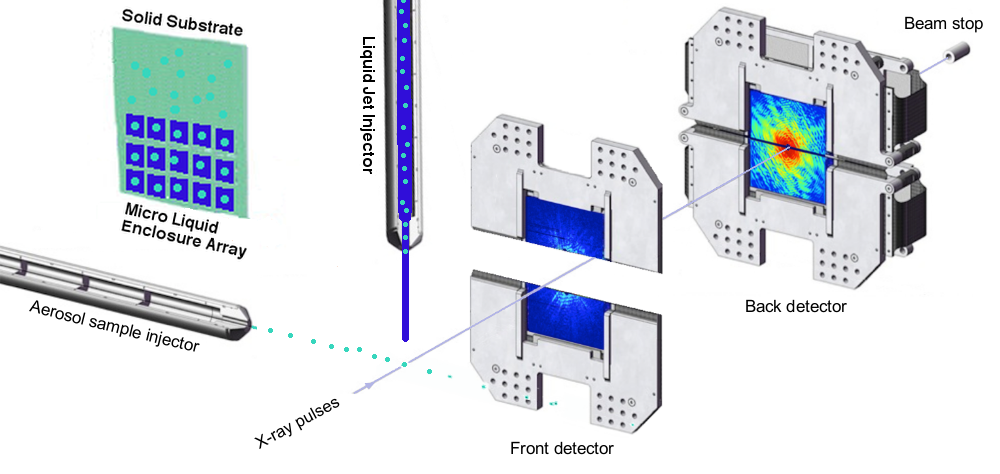
\includegraphics[width=90mm]{Chapter_04_ExperimentalGeometry.png}
\caption{Experimental geometry, including different sample delivery system. From the bottom left the x-rays pulses enter the chamber. The experimentalist can now select a sample delivery system. Shown are an aerosol sample delivery system, liquid jet injection system, and two types of substrate bound sample delivery systems. If the beam intersect the sample (and/or substrate) a diffraction pattern is recorded on two sets of detectors, placed at different distances from the interaction region.}
\end{figure}

\section{Substrate-bound Sample Delivery}
\subsection{Solid substrate}
One of the easiest ways of introducing samples is by attaching them to a solid surface. Shortly after the operation of the first XFEL (FLASH) the principle of diffract-before-destroy was demonstrated on a inorganic sample attached to a fixed membrane [Chapman]. Soon after the first cells were imaged on a silicon-nitrate window. The main disadvantages of this sample delivery system are i)the sample has to be able to tolerate prolonged exposure to reduced pressure, ii) the substrate causes significant background scattering, and iii) the repetition rate is limited by the time it takes to mechanically move the solid substrate from one position to the next. The latter becomes a significant problem at the high repetition rate XFEL sources.

\subsection{Micro Compartments}
In order to circumvent the problem of the prolonged exposure to the vacuum, a system called Micro Liquid Enclosure Array (MLEA) can be used. A MLEA system consists of an array of micro-compartments filled with liquid attached to a regular grid (see figure \ref{fig:experimental_geometry}. The microcompartments are closed off with by a membrane. This method has been successfully used in the imaging of cells. Getting your sample into the microcompartments is tedious and time consuming. The liquid in the microcompartments produces significant background scattering. 

\subsection{Liquid Jets}

Liquid jet systems can produce stable streams of particles in solution. Mainly two types of liquid jet nozzles are used for sample injection into the XFEL pulse train: i) liquid nozzles (Rayleigh jets), ii) liquid nozzles assisted by coaxial gas flow also referred to as gas dynamic virtual nozzle (GDVN). 

Vacuum compatible systems of the Rayleigh jets with diameters ranging approximately from 5 to 100 $\mu m$
exist. Typical liquid flow velocities of such jets is 120 m/s. The sample consumption within such a jet is in the order of ml/s. For many biological samples this rate of sample consumption is too high. Sample consumption can be reduced by slowing down the stream or by reducing the diameter of the nozzle. However, for orifice diameters smaller than 10 $\mu m$, clogging of the nozzles becomes a serious issue. To reduce the jet diameter without the danger of clogging the sample delivery, GDVN liquid jets were introduced [DePonte]. In a GDVN nozzle a coaxial stream of high velocity He gas is used to accelerate the liquid stream. Similar to the flow of water from a tab, the accelerating stream is reduced in diameter. Jet diameters below 1 $\mu m$ have been recently achieved [W]. 

Liquid jets have the advantage to study biological samples in their natural environment, to refresh the sample throughout the experiment with sample consumption in the order of 10 $\mu l$/min [Weierstall 2012], and allows for imaging at high repetition rates. This GDVN setup is commonly used in serial femtosecond crystallography (SFX) experiments. The Bragg peaks of nano crystals are sufficiently strong to surmount the background scattering from the surrounding jet.

\section{Substrate-free sample delivery}
In FXI everything that is illuminated by the X-ray pulse is sample, including the structure of the sample holder, the liquid column of a liquid jet, or materials that make up microfluidic devices. Such sample holders contribute to scattering and increase unwanted noise. Especially for weakly scattering single particles the noise might drown the signal. Aerosol injection removes this clutter and assures that the sample is clearly isolated from its surroundings, and this is, as we see in a later chapter, important for image recovery.

An aerosol injector produces small droplets of particles dissolved in a volatile buffer, typically ammonium acetate. The buffer evaporates under the reduced pressure, ideally leaving behind only the particle. There are two main types of nozzles that can be used to produce small drops: the Gas Dynamic Virtual Nozzle, and electro spray ionisation (ESI).

\subsection{Gas Dynamic Virtual Nozzle}

If the coaxial flow of gas creates a jet with a diameter smaller than then a characteristic $d_j$ the surface tension in the liquid will cause the jet to break up into a mist of small droplets. $d_j$ can be estimated on the basis of energy conservation, and is a function of the effective pressure drop $\Delta P$. It is assumed that all energy is transformed to kinetic energy [Calvo].
\begin{equation}
d_j^{(GDVN)} = 2 \sqrt{Q \cdot \left(\frac{\rho}{2 \pi^2 \Delta P}\right)^{1/2}}
\end{equation}    
$Q$ denotes the flow rate and $\rho$ is the density of the liquid. The final drop diameter $d_d$ can be related to the jet diameter using the ratio $d_d / d_j \approx 1.9$, which is the classical Rayleigh breakup []. Empirically this assumption has shown to work well for low viscosity media such as water. The GDVN can create droplets in the size range of 400 nm - 2000 nm. Sample consumption is in the range of ul/min.

\subsection{Aerodynamic Lens Stack}
After the droplets formed, they start to evaporate in the reduced pressure environment, leaving only the non-volatile particles in the 'drop'. The aerosolised particles are guided into an aerodynamic lens stack (see figure ). This is a series of cylindrical cavities, connected by co-aligned orifices, that collimate the droplets into a narrow beam of particles [].

For robust particles, which are large compared to the drop size, this type of sample injection has shown to be very successful. This sample injection method really opened up the possibility to measure the diffraction pattern of isolated single particles at high signal-to-noise ratios at very high repetition rates. Up to 80\% hit ratios of the 120 Hz repetition rates of the LCLS have been recorded [Hantke]. The results discussed in this thesis come from datasets that were generated using the GVDN injection method.

For many samples aerosol injection is not disruptive. Molecular dynamics simulation have shown that the conformation of proteins is conserved up till the moment that the last structural water evaporates[]. For the cyanobacterial cells described in this paper it has been shown that the shape and the autofluorescence properties of the cell membranes of the injected cells remain unchanged [PAPER I]. This is not quite unexpected. Aerosols of cyanobacteria can be carried for long distances, and metabolically active cells have been detected at altitudes of 20-70 km where atmospheric pressure drops to below a millibar []. Other sample cell lines such as E coli and brewers yeast, or many types of viruses have shown to be viable after injection. Nevertheless, not all sample types may be amenable to aerosol sample injection, and any sample type should be tested prior to experiments.  

\subsection{Electro Spray Ionisation}
Over the last years it became apparent that GDVN sample injection does have its limitations. If the particle becomes small compared to the drop size, wide size distributions of otherwise uniformly sized particles were measured [Daurer, Hantke]. These observations might be explained by a combination of an incomplete evaporation process, and the build up a significant shell of debris, originating from impurities present in the solution, around the particle. To purify the measured sample, smaller drops had to be generated. A common aerosolisation technique used in mass spectrometry called electro spray ionisation (ESI) is known to be able to produce small droplets.

ESI nozzles produce droplets through a similar droplet formation process as occurs in the GDVN. The difference lies in the process that drives jet acceleration. In ESI the jet is accelerated by an externally applied electrostatic potential. In the capillary the solvent (volatile buffer) is mixed with negatively charged ions. By applying an external field these ions are accelerated, accelerating the entire jet. The accelerated jet will ultimately break into small drops similar as happens in a GDVN. The characteristic $d_j^{ESI}$ can be described as a function of the surface tension $\sigma$, vacuum permittivity $\varepsilon_0$, electrical conductivity $C$, as well as the flow rate and the density of the liquid.
\begin{equation}
d_j^{(ESI)} \approx 2 \sqrt{Q \cdot \left(\frac{\rho \varepsilon_0}{\sigma C}\right)^{1/3}}
\end{equation}

After the process of evaporation initiates an electric potential starts to further build up in the drops, eventually leading to a coulomb explosions of the drops [Cole]. Cycles of evarporation and explosion leads to smaller and smaller drops. Initial experiments showed that drops of mono disperse droplets of size 150-200 nm can be generated with ESI. ESI can be combined with an aerodynamic lens stack as well. 

The transfer of ESI to FXI is a considerable achievement that will allow the field to move forward to image smaller particles such as proteins. This would not have been possible using the GDVN aerosolisation. ESI has been shown to also function under lower flowrates, allowing to reduce sample consumption to 10 nl/min []. This sample consumption rate is compatible with samples that are only available in small quantities. 

\subsection{Drop-on-demand}
The combination of ESI and a quadrupole with an ion trap for storage allows for a pulsed delivery system that can be tuned to match the repetition rate of the XFEL. This is generally referred to as drop-on-demand. This would reduce the sample consumption even further. Moreover the ion trap can also be utilized for sample selection prior to injection of sample into the x-ray pulse. This is important for single proteins as they scatter very little signal, which makes it very difficult to separate diffraction patterns from the real particle from diffraction patterns from potential contamination. 

